% Options for packages loaded elsewhere
\PassOptionsToPackage{unicode}{hyperref}
\PassOptionsToPackage{hyphens}{url}
%
\documentclass[
]{article}
\usepackage{amsmath,amssymb}
\usepackage{lmodern}
\usepackage{iftex}
\ifPDFTeX
  \usepackage[T1]{fontenc}
  \usepackage[utf8]{inputenc}
  \usepackage{textcomp} % provide euro and other symbols
\else % if luatex or xetex
  \usepackage{unicode-math}
  \defaultfontfeatures{Scale=MatchLowercase}
  \defaultfontfeatures[\rmfamily]{Ligatures=TeX,Scale=1}
\fi
% Use upquote if available, for straight quotes in verbatim environments
\IfFileExists{upquote.sty}{\usepackage{upquote}}{}
\IfFileExists{microtype.sty}{% use microtype if available
  \usepackage[]{microtype}
  \UseMicrotypeSet[protrusion]{basicmath} % disable protrusion for tt fonts
}{}
\makeatletter
\@ifundefined{KOMAClassName}{% if non-KOMA class
  \IfFileExists{parskip.sty}{%
    \usepackage{parskip}
  }{% else
    \setlength{\parindent}{0pt}
    \setlength{\parskip}{6pt plus 2pt minus 1pt}}
}{% if KOMA class
  \KOMAoptions{parskip=half}}
\makeatother
\usepackage{xcolor}
\usepackage[margin=1in]{geometry}
\usepackage{color}
\usepackage{fancyvrb}
\newcommand{\VerbBar}{|}
\newcommand{\VERB}{\Verb[commandchars=\\\{\}]}
\DefineVerbatimEnvironment{Highlighting}{Verbatim}{commandchars=\\\{\}}
% Add ',fontsize=\small' for more characters per line
\usepackage{framed}
\definecolor{shadecolor}{RGB}{248,248,248}
\newenvironment{Shaded}{\begin{snugshade}}{\end{snugshade}}
\newcommand{\AlertTok}[1]{\textcolor[rgb]{0.94,0.16,0.16}{#1}}
\newcommand{\AnnotationTok}[1]{\textcolor[rgb]{0.56,0.35,0.01}{\textbf{\textit{#1}}}}
\newcommand{\AttributeTok}[1]{\textcolor[rgb]{0.77,0.63,0.00}{#1}}
\newcommand{\BaseNTok}[1]{\textcolor[rgb]{0.00,0.00,0.81}{#1}}
\newcommand{\BuiltInTok}[1]{#1}
\newcommand{\CharTok}[1]{\textcolor[rgb]{0.31,0.60,0.02}{#1}}
\newcommand{\CommentTok}[1]{\textcolor[rgb]{0.56,0.35,0.01}{\textit{#1}}}
\newcommand{\CommentVarTok}[1]{\textcolor[rgb]{0.56,0.35,0.01}{\textbf{\textit{#1}}}}
\newcommand{\ConstantTok}[1]{\textcolor[rgb]{0.00,0.00,0.00}{#1}}
\newcommand{\ControlFlowTok}[1]{\textcolor[rgb]{0.13,0.29,0.53}{\textbf{#1}}}
\newcommand{\DataTypeTok}[1]{\textcolor[rgb]{0.13,0.29,0.53}{#1}}
\newcommand{\DecValTok}[1]{\textcolor[rgb]{0.00,0.00,0.81}{#1}}
\newcommand{\DocumentationTok}[1]{\textcolor[rgb]{0.56,0.35,0.01}{\textbf{\textit{#1}}}}
\newcommand{\ErrorTok}[1]{\textcolor[rgb]{0.64,0.00,0.00}{\textbf{#1}}}
\newcommand{\ExtensionTok}[1]{#1}
\newcommand{\FloatTok}[1]{\textcolor[rgb]{0.00,0.00,0.81}{#1}}
\newcommand{\FunctionTok}[1]{\textcolor[rgb]{0.00,0.00,0.00}{#1}}
\newcommand{\ImportTok}[1]{#1}
\newcommand{\InformationTok}[1]{\textcolor[rgb]{0.56,0.35,0.01}{\textbf{\textit{#1}}}}
\newcommand{\KeywordTok}[1]{\textcolor[rgb]{0.13,0.29,0.53}{\textbf{#1}}}
\newcommand{\NormalTok}[1]{#1}
\newcommand{\OperatorTok}[1]{\textcolor[rgb]{0.81,0.36,0.00}{\textbf{#1}}}
\newcommand{\OtherTok}[1]{\textcolor[rgb]{0.56,0.35,0.01}{#1}}
\newcommand{\PreprocessorTok}[1]{\textcolor[rgb]{0.56,0.35,0.01}{\textit{#1}}}
\newcommand{\RegionMarkerTok}[1]{#1}
\newcommand{\SpecialCharTok}[1]{\textcolor[rgb]{0.00,0.00,0.00}{#1}}
\newcommand{\SpecialStringTok}[1]{\textcolor[rgb]{0.31,0.60,0.02}{#1}}
\newcommand{\StringTok}[1]{\textcolor[rgb]{0.31,0.60,0.02}{#1}}
\newcommand{\VariableTok}[1]{\textcolor[rgb]{0.00,0.00,0.00}{#1}}
\newcommand{\VerbatimStringTok}[1]{\textcolor[rgb]{0.31,0.60,0.02}{#1}}
\newcommand{\WarningTok}[1]{\textcolor[rgb]{0.56,0.35,0.01}{\textbf{\textit{#1}}}}
\usepackage{longtable,booktabs,array}
\usepackage{calc} % for calculating minipage widths
% Correct order of tables after \paragraph or \subparagraph
\usepackage{etoolbox}
\makeatletter
\patchcmd\longtable{\par}{\if@noskipsec\mbox{}\fi\par}{}{}
\makeatother
% Allow footnotes in longtable head/foot
\IfFileExists{footnotehyper.sty}{\usepackage{footnotehyper}}{\usepackage{footnote}}
\makesavenoteenv{longtable}
\usepackage{graphicx}
\makeatletter
\def\maxwidth{\ifdim\Gin@nat@width>\linewidth\linewidth\else\Gin@nat@width\fi}
\def\maxheight{\ifdim\Gin@nat@height>\textheight\textheight\else\Gin@nat@height\fi}
\makeatother
% Scale images if necessary, so that they will not overflow the page
% margins by default, and it is still possible to overwrite the defaults
% using explicit options in \includegraphics[width, height, ...]{}
\setkeys{Gin}{width=\maxwidth,height=\maxheight,keepaspectratio}
% Set default figure placement to htbp
\makeatletter
\def\fps@figure{htbp}
\makeatother
\setlength{\emergencystretch}{3em} % prevent overfull lines
\providecommand{\tightlist}{%
  \setlength{\itemsep}{0pt}\setlength{\parskip}{0pt}}
\setcounter{secnumdepth}{-\maxdimen} % remove section numbering
\ifLuaTeX
  \usepackage{selnolig}  % disable illegal ligatures
\fi
\IfFileExists{bookmark.sty}{\usepackage{bookmark}}{\usepackage{hyperref}}
\IfFileExists{xurl.sty}{\usepackage{xurl}}{} % add URL line breaks if available
\urlstyle{same} % disable monospaced font for URLs
\hypersetup{
  pdftitle={Práctica dirigida 7},
  hidelinks,
  pdfcreator={LaTeX via pandoc}}

\title{Práctica dirigida 7}
\author{}
\date{\vspace{-2.5em}}

\begin{document}
\maketitle

{
\setcounter{tocdepth}{2}
\tableofcontents
}
\textbf{FACULTAD DE CIENCIAS SOCIALES - PUCP}

\hypertarget{curso-pol-278---estaduxedstica-para-el-anuxe1lisis-poluxedtico-1-semestre-2025---1}{%
\subsection{\texorpdfstring{Curso: POL 278 - Estadística para el
análisis político 1 \textbar{} Semestre 2025 - 1
}{Curso: POL 278 - Estadística para el análisis político 1 \textbar{} Semestre 2025 - 1  }}\label{curso-pol-278---estaduxedstica-para-el-anuxe1lisis-poluxedtico-1-semestre-2025---1}}

\begin{center}\rule{0.5\linewidth}{0.5pt}\end{center}

\hypertarget{diagramas-de-dispersiuxf3n-y-correlaciuxf3n}{%
\subsection{\texorpdfstring{\textbf{Diagramas de dispersión y
correlación}}{Diagramas de dispersión y correlación}}\label{diagramas-de-dispersiuxf3n-y-correlaciuxf3n}}

\hypertarget{ideas-clave}{%
\subsubsection{Ideas clave}\label{ideas-clave}}

La correlación es en esencia una medida normalizada de asociación o
covariación lineal entre dos variables.

\begin{itemize}
\item
  La \textbf{correlación} es una medida de la relación (covariación)
  entre \textbf{dos variables cuantitativas.}
\item
  La manera más sencilla de saber si dos variables están correlacionadas
  es determinar si co-varían (varían conjuntamente).
\item
  Es importante hacer notar que \textbf{esta covariación o relación no
  implica necesariamente causalidad}: La correlación puede ser fortuita,
  como en el caso clásico de la correlación entre el número de venta de
  helados e incendios, debido al efecto de una tercera variable, la
  temperatura ambiental. A este tipo de relación se le llama
  ``espuria''.
\end{itemize}

\hypertarget{hipuxf3tesis-de-la-prueba-de-correlaciuxf3n}{%
\subsubsection{Hipótesis de la prueba de
correlación}\label{hipuxf3tesis-de-la-prueba-de-correlaciuxf3n}}

\begin{itemize}
\tightlist
\item
  H0 : No existe correlación entre las variables
\item
  H1 : Existe correlación entre las variables
\end{itemize}

\hypertarget{coeficiente-de-correlaciuxf3n-de-pearson}{%
\subsubsection{Coeficiente de Correlación de
Pearson}\label{coeficiente-de-correlaciuxf3n-de-pearson}}

\begin{itemize}
\item
  ``El Coeficiente de Correlación de Pearson es un estadístico
  paramétrico, pues se asume que ambas variables tienen una distribución
  aproximadamente normal, o sea, distribución normal bivariante''.
\item
  Es una medida que \textbf{puede variar entre -1 y +1}, ambos extremos
  indicando correlaciones perfectas, negativa y positiva
  respectivamente.
\item
  Un valor de r = 0 indica que no existe relación lineal entre las dos
  variables.
\end{itemize}

\hypertarget{aplicaciuxf3n-pruxe1ctica}{%
\subsubsection{Aplicación práctica}\label{aplicaciuxf3n-pruxe1ctica}}

\hypertarget{pregunta-de-investigaciuxf3n}{%
\section{Pregunta de investigación}\label{pregunta-de-investigaciuxf3n}}

¿Cómo se relaciona la percepción de corrupción con los indicadores de
democracia de los países? 🤔

Para la sesión de hoy trabajaremos con una base de datos que contiene
variables obtenidas de las siguientes bases: - Freedom in the World -
V-Dem - Democracy Index - Global Corruption Barometer

\textbf{Información sobre las bases:}

\begin{itemize}
\item
  Freedom in the World es elaborado por Freedom House y analiza los
  siguientes aspectos: el proceso electoral, las políticas
  pluriculturales y la participación, el funcionamiento del gobierno, la
  libertad de expresión y de creencia, los derechos de asociación y
  organización, el estado de derecho, la autonomía personal y los
  derechos individuales.
\item
  V-Dem es publicada por el V-Dem Institute. En ella se describe la
  calidad de los gobiernos a partir de información de 542 indicadores.
  La data describe todos los aspectos de un gobierno, brindándo énfasis
  en la calidad de la democracia, la inclusividad y otros indicadores
  económicos.
\item
  Democracy Index es elaborado por The Economist y utiliza 60
  indicadores, agrupados en cinco categorías: proceso electoral y
  pluralismo, libertades civiles, funcionamiento del gobierno,
  participación política y política cultural. A partir de estas
  categorías posiciona a los países en alguno de los cuatro tipos de
  régimen: Democracia plena, democracia imperfecta, régimen híbrido y
  régimen autoritario.
\item
  Global Corruption Barometer es publicado por Transparencia
  Internacional y contiene información proveniente de la opinión pública
  ciudadana
\end{itemize}

Las variables que usaermos en la presente sesión son las siguientes:

\begin{itemize}
\tightlist
\item
  \emph{Pais:} nombre del país analizado.
\item
  \emph{c\_funcionarios:} percepción sobre la corrupción de funcionarios
  en el pais.
\item
  \emph{Democracia:} indicador de democracia en el país.
\item
  \emph{c\_diferencia:} percepción de que la ciudadanía puede hacer la
  diferencia en la lucha contra la corrupción
\item
  \emph{Fun\_gob:} indicador sobre el funcionamiento del gobierno del
  país.
\end{itemize}

\hypertarget{cargamos-nuestra-base-de-datos}{%
\subsubsection{Cargamos nuestra base de
datos:}\label{cargamos-nuestra-base-de-datos}}

\begin{Shaded}
\begin{Highlighting}[]
\FunctionTok{library}\NormalTok{(rio)}
\FunctionTok{library}\NormalTok{(dplyr)}
\FunctionTok{library}\NormalTok{(ggplot2)}

\NormalTok{data}\OtherTok{=}\FunctionTok{import}\NormalTok{(}\StringTok{"corrupcion{-}democracia{-}1.xlsx"}\NormalTok{)}
\FunctionTok{names}\NormalTok{(data)}
\end{Highlighting}
\end{Shaded}

\begin{verbatim}
##  [1] "Pais"           "c_aumento"      "c_presi"       
##  [4] "c_congreso"     "c_funcionarios" "c_local"       
##  [7] "c_policia"      "c_relig"        "c_nolucha"     
## [10] "c_diferencia"   "c_frase1"       "c_frase2"      
## [13] "c_frase3"       "Poli"           "Part"          
## [16] "Libertad"       "Der_pol"        "Lib_civiles"   
## [19] "Democracia"     "Proceso_elect"  "Fun_gob"       
## [22] "Part_poli"
\end{verbatim}

\hypertarget{ejercicio-1-existe-relaciuxf3n-entre-el-indicador-de-democracia-y-el-porcentaje-de-personas-que-perciben-que-los-funcionario-son-corruptos-en-el-pauxeds}{%
\subsubsection{Ejercicio 1: ¿Existe relación entre el indicador de
democracia y el porcentaje de personas que perciben que los funcionario
son corruptos en el
país?}\label{ejercicio-1-existe-relaciuxf3n-entre-el-indicador-de-democracia-y-el-porcentaje-de-personas-que-perciben-que-los-funcionario-son-corruptos-en-el-pauxeds}}

\textbf{Paso 1: Exploramos variables de interés}

Primero analicemos la variable \textbf{c\_funcionarios}:

\begin{Shaded}
\begin{Highlighting}[]
\FunctionTok{str}\NormalTok{(data}\SpecialCharTok{$}\NormalTok{c\_funcionarios)}
\end{Highlighting}
\end{Shaded}

\begin{verbatim}
##  num [1:118] 0.45 0.39 0.277 0.45 0.12 ...
\end{verbatim}

Análisis descriptivo de la variable \textbf{c\_funcionarios}:

\begin{Shaded}
\begin{Highlighting}[]
\NormalTok{data }\SpecialCharTok{\%\textgreater{}\%}
 \FunctionTok{summarize}\NormalTok{(}\AttributeTok{Min =} \FunctionTok{min}\NormalTok{(c\_funcionarios, }\AttributeTok{na.rm =} \ConstantTok{TRUE}\NormalTok{),}
           \AttributeTok{Media =} \FunctionTok{mean}\NormalTok{(c\_funcionarios, }\AttributeTok{na.rm =} \ConstantTok{TRUE}\NormalTok{),}
           \AttributeTok{Mediana =} \FunctionTok{median}\NormalTok{(c\_funcionarios, }\AttributeTok{na.rm =} \ConstantTok{TRUE}\NormalTok{),}
           \AttributeTok{Max =} \FunctionTok{max}\NormalTok{(c\_funcionarios, }\AttributeTok{na.rm =} \ConstantTok{TRUE}\NormalTok{))}
\end{Highlighting}
\end{Shaded}

\begin{verbatim}
##    Min     Media   Mediana  Max
## 1 0.06 0.3480088 0.3200429 0.79
\end{verbatim}

Ahora, analicemos nuestra segunda variable \textbf{Democracia}:

\begin{Shaded}
\begin{Highlighting}[]
\FunctionTok{str}\NormalTok{(data}\SpecialCharTok{$}\NormalTok{Democracia)}
\end{Highlighting}
\end{Shaded}

\begin{verbatim}
##  num [1:118] 5.98 3.56 6.96 4.11 9.09 2.65 3.13 7.78 5.61 5.49 ...
\end{verbatim}

Análisis descriptivo de la variable \textbf{Democracia}:

\begin{Shaded}
\begin{Highlighting}[]
\NormalTok{data }\SpecialCharTok{\%\textgreater{}\%}
 \FunctionTok{summarize}\NormalTok{(}\AttributeTok{Min =} \FunctionTok{min}\NormalTok{(Democracia, }\AttributeTok{na.rm =} \ConstantTok{TRUE}\NormalTok{),}
           \AttributeTok{Media =} \FunctionTok{mean}\NormalTok{(Democracia, }\AttributeTok{na.rm =} \ConstantTok{TRUE}\NormalTok{),}
           \AttributeTok{Mediana =} \FunctionTok{median}\NormalTok{(Democracia, }\AttributeTok{na.rm =} \ConstantTok{TRUE}\NormalTok{),}
           \AttributeTok{Max =} \FunctionTok{max}\NormalTok{(Democracia, }\AttributeTok{na.rm =} \ConstantTok{TRUE}\NormalTok{))}
\end{Highlighting}
\end{Shaded}

\begin{verbatim}
##    Min    Media Mediana  Max
## 1 1.93 5.852368    6.23 9.39
\end{verbatim}

\textbf{Paso 2: Gráfico de dispersión}

Visualizamos la relación entre dos variables cuantitativas. Esta
``nube'' de puntos en el gráfico de dispersión nos da una idea visual
(preliminar) de la probable relación entre las variables.

\begin{Shaded}
\begin{Highlighting}[]
\FunctionTok{ggplot}\NormalTok{(data, }\FunctionTok{aes}\NormalTok{(}\AttributeTok{x=}\NormalTok{c\_funcionarios, }\AttributeTok{y=}\NormalTok{Democracia)) }\SpecialCharTok{+}
  \FunctionTok{geom\_point}\NormalTok{(}\AttributeTok{colour=}\StringTok{"skyblue"}\NormalTok{) }\SpecialCharTok{+}  \FunctionTok{xlab}\NormalTok{(}\StringTok{"\% de personas que opinan que los funcionarios del }\SpecialCharTok{\textbackslash{}n}\StringTok{ gobierno están envueltos en corrupción"}\NormalTok{) }\SpecialCharTok{+}  \FunctionTok{ylab}\NormalTok{(}\StringTok{"Puntaje de democracia"}\NormalTok{) }\SpecialCharTok{+}
  \FunctionTok{ggtitle}\NormalTok{(}\StringTok{"Relación entre la percepción de corrupción }\SpecialCharTok{\textbackslash{}n}\StringTok{ de funcionarios del gobierno y la democracia"}\NormalTok{) }\SpecialCharTok{+}
  \FunctionTok{theme\_light}\NormalTok{()}\SpecialCharTok{+} \FunctionTok{geom\_smooth}\NormalTok{(}\AttributeTok{method=}\NormalTok{lm,}\AttributeTok{se=}\NormalTok{F)}
\end{Highlighting}
\end{Shaded}

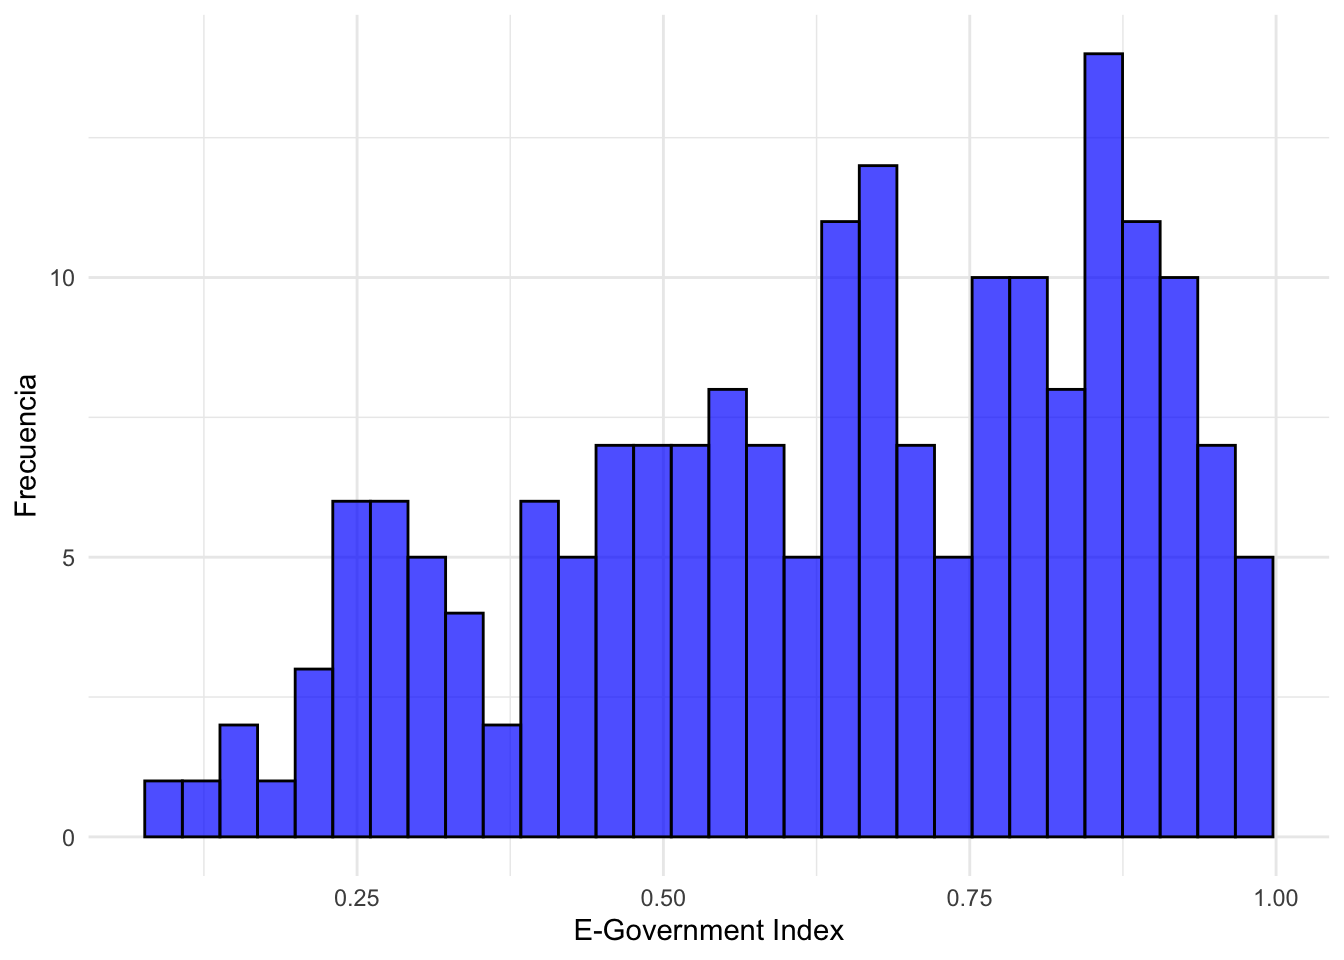
\includegraphics{semana9_practica_files/figure-latex/unnamed-chunk-6-1.pdf}

¿Qué nos indica el gráfico? ¿Existirá correlación? ¿Con qué fuerza? ¿Qué
sentido?

El gráfico nos indica una correlación negativa. Adicionalmente, es
posible asociar la distribución de los puntos con una correlación
pequeña o mediana. ¿Cómo sabremos la fuerza de la correlación? Con la
\textbf{prueba de correlación}

\textbf{Paso 3: Correlación}

Dos hipótesis:

\begin{itemize}
\tightlist
\item
  H0 = No existe correlación entre el porcentaje de personas que opinan
  que los funcionarios del gobierno están envueltos en corrupción y el
  puntaje de la democracia
\item
  H1 = Sí existe correlación entre el porcentaje de personas que opinan
  que los funcionarios del gobierno están envueltos en corrupción y el
  puntaje de la democracia
\end{itemize}

\begin{Shaded}
\begin{Highlighting}[]
\CommentTok{\#Prueba de correlación}
\FunctionTok{cor.test}\NormalTok{(data}\SpecialCharTok{$}\NormalTok{Democracia, data}\SpecialCharTok{$}\NormalTok{c\_funcionarios)}
\end{Highlighting}
\end{Shaded}

\begin{verbatim}
## 
##  Pearson's product-moment correlation
## 
## data:  data$Democracia and data$c_funcionarios
## t = -3.3754, df = 112, p-value = 0.001014
## alternative hypothesis: true correlation is not equal to 0
## 95 percent confidence interval:
##  -0.4619594 -0.1270461
## sample estimates:
##       cor 
## -0.303861
\end{verbatim}

\begin{itemize}
\tightlist
\item
  p \textless{} 0.05 Rechazas la H0 (por lo tanto, sí hay correlación)
\item
  P \textgreater{} 0.05 No rechazas la H0
\end{itemize}

\textbf{¿Qué nos dice el resultado?} \emph{Recuerda que en la
interpretación no debe faltar: (i) intepretación del p-valor y (ii)
interpretación del coeficiente de correlación (cor)}

\textbf{Reporte:} Dado que el p-valor es menor a 0.05, rechazamos la H0.
Por lo tanto, podemos afirmar que \textbf{existe correlación} entre el
porcentaje de personas que opinan que los funcionarios del gobierno
están envueltos en corrupción y el indicador de la democracia.

El coeficiente es de -0.30, lo que quiere decir: (i) Se trata de una
\textbf{correlación negativa}; es decir, relación indirecta (-) y (ii)
Según los criterios de Cohen (1988), se trata de una correlación
mediana.

En síntesis, se espera que mientras más personas perciban que la
corrupción es alta, menor será el apoyo a la democracia.

Sin embargo, esta relación es de fuerza media, lo que significa que
aunque la tendencia es clara, no es una relación extremadamente fuerte,
pero sí lo suficientemente significativa como para ser considerada
relevante.

\textbf{Interpretación} Esta relación inversa se puede deber a la menor
confianza en la institucionalidad democrática, asociándola con actos de
corrupción.

\hypertarget{ejercicio-2-existe-relaciuxf3n-entre-el-indicador-de-funcionamiento-de-gobierno-y-el-porcentaje-de-personas-que-creen-que-los-ciudadanos-pueden-hacer-la-diferencia-en-la-lucha-contra-la-corrupciuxf3n}{%
\subsubsection{Ejercicio 2: ¿Existe relación entre el indicador de
funcionamiento de gobierno y el porcentaje de personas que creen que los
ciudadanos pueden hacer la diferencia en la lucha contra la
corrupción?}\label{ejercicio-2-existe-relaciuxf3n-entre-el-indicador-de-funcionamiento-de-gobierno-y-el-porcentaje-de-personas-que-creen-que-los-ciudadanos-pueden-hacer-la-diferencia-en-la-lucha-contra-la-corrupciuxf3n}}

\textbf{Paso 1: Exploramos variables de interés}

Primero analicemos la variable \textbf{c\_diferencia}:

\begin{Shaded}
\begin{Highlighting}[]
\FunctionTok{str}\NormalTok{(data}\SpecialCharTok{$}\NormalTok{c\_diferencia)}
\end{Highlighting}
\end{Shaded}

\begin{verbatim}
##  num [1:118] 0.57 0.5 0.65 0.29 0.8 0.33 0.1 0.53 0.42 0.63 ...
\end{verbatim}

Análisis descriptivo de la variable \textbf{c\_diferencia}:

\begin{Shaded}
\begin{Highlighting}[]
\NormalTok{data }\SpecialCharTok{\%\textgreater{}\%}
 \FunctionTok{summarize}\NormalTok{(}\AttributeTok{Min =} \FunctionTok{min}\NormalTok{(c\_diferencia, }\AttributeTok{na.rm =} \ConstantTok{TRUE}\NormalTok{),}
           \AttributeTok{Media =} \FunctionTok{mean}\NormalTok{(c\_diferencia, }\AttributeTok{na.rm =} \ConstantTok{TRUE}\NormalTok{),}
           \AttributeTok{Mediana =} \FunctionTok{median}\NormalTok{(c\_diferencia, }\AttributeTok{na.rm =} \ConstantTok{TRUE}\NormalTok{),}
           \AttributeTok{Max =} \FunctionTok{max}\NormalTok{(c\_diferencia, }\AttributeTok{na.rm =} \ConstantTok{TRUE}\NormalTok{))}
\end{Highlighting}
\end{Shaded}

\begin{verbatim}
##   Min     Media Mediana  Max
## 1 0.1 0.5436752    0.55 0.83
\end{verbatim}

Ahora, analicemos nuestra segunda variable \textbf{Fun\_gob}:

\begin{Shaded}
\begin{Highlighting}[]
\FunctionTok{str}\NormalTok{(data}\SpecialCharTok{$}\NormalTok{Fun\_gob)}
\end{Highlighting}
\end{Shaded}

\begin{verbatim}
##  num [1:118] 4.71 2.21 5 2.86 8.93 2.14 2.86 8.93 5.36 4.64 ...
\end{verbatim}

Análisis descriptivo de la variable \textbf{Fun\_gob}:

\begin{Shaded}
\begin{Highlighting}[]
\NormalTok{data }\SpecialCharTok{\%\textgreater{}\%}
 \FunctionTok{summarize}\NormalTok{(}\AttributeTok{Min =} \FunctionTok{min}\NormalTok{(Fun\_gob, }\AttributeTok{na.rm =} \ConstantTok{TRUE}\NormalTok{),}
           \AttributeTok{Media =} \FunctionTok{mean}\NormalTok{(Fun\_gob, }\AttributeTok{na.rm =} \ConstantTok{TRUE}\NormalTok{),}
           \AttributeTok{Mediana =} \FunctionTok{median}\NormalTok{(Fun\_gob, }\AttributeTok{na.rm =} \ConstantTok{TRUE}\NormalTok{),}
           \AttributeTok{Max =} \FunctionTok{max}\NormalTok{(Fun\_gob, }\AttributeTok{na.rm =} \ConstantTok{TRUE}\NormalTok{))}
\end{Highlighting}
\end{Shaded}

\begin{verbatim}
##   Min    Media Mediana  Max
## 1   0 5.176754    5.36 9.64
\end{verbatim}

\textbf{Paso 2: Gráfico de dispersión}

\begin{Shaded}
\begin{Highlighting}[]
\FunctionTok{ggplot}\NormalTok{(data, }\FunctionTok{aes}\NormalTok{(}\AttributeTok{x=}\NormalTok{c\_diferencia, }\AttributeTok{y=}\NormalTok{Fun\_gob)) }\SpecialCharTok{+}
  \FunctionTok{geom\_point}\NormalTok{(}\AttributeTok{colour=}\StringTok{"skyblue"}\NormalTok{) }\SpecialCharTok{+}  \FunctionTok{xlab}\NormalTok{(}\StringTok{"\% de personas que creen que los ciudadanos }\SpecialCharTok{\textbackslash{}n}\StringTok{ pueden hacer la diferencia en la lucha contra la corrupción"}\NormalTok{) }\SpecialCharTok{+}  \FunctionTok{ylab}\NormalTok{(}\StringTok{"Indicador de funcionamiento de gobierno"}\NormalTok{) }\SpecialCharTok{+}
  \FunctionTok{theme\_light}\NormalTok{()}\SpecialCharTok{+} \FunctionTok{geom\_smooth}\NormalTok{(}\AttributeTok{method=}\NormalTok{lm,}\AttributeTok{se=}\NormalTok{F)}
\end{Highlighting}
\end{Shaded}

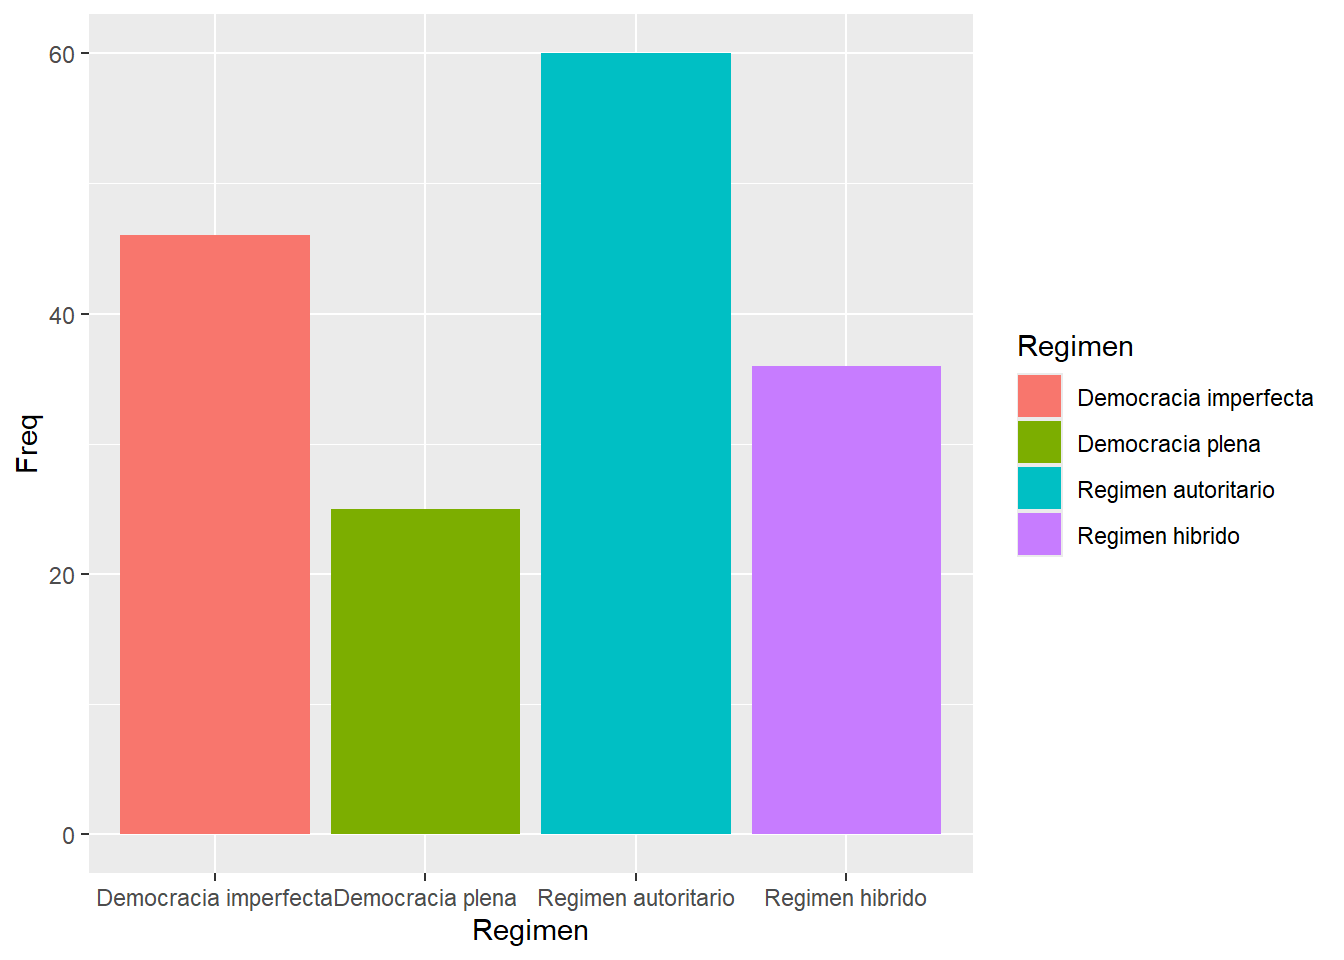
\includegraphics{semana9_practica_files/figure-latex/unnamed-chunk-12-1.pdf}

¿Qué nos indica el gráfico? ¿Existirá correlación? ¿Con qué fuerza? ¿Qué
sentido?

El gráfico nos indica una correlación positiva. Posiblemente se trate de
una correlación pequeña, pero no lo sabremos con certeza hasta realizar
la \textbf{prueba de correlación}

\textbf{Paso 3: Correlación}

Dos hipótesis:

\begin{itemize}
\tightlist
\item
  H0 = No existe correlación entre el el indicador de funcionamiento del
  gobierno y el porcentaje de personas que creen que los ciudadanos
  pueden hacer la diferencia en la lucha contra la corrupción
\item
  H1 = Sí existe correlación entre el indicador de funcionamiento del
  gobierno y el porcentaje de personas que creen que los ciudadanos
  pueden hacer la diferencia en la lucha contra la corrupción
\end{itemize}

\begin{Shaded}
\begin{Highlighting}[]
\CommentTok{\#Prueba de correlación}
\FunctionTok{cor.test}\NormalTok{(data}\SpecialCharTok{$}\NormalTok{c\_diferencia, data}\SpecialCharTok{$}\NormalTok{Fun\_gob)}
\end{Highlighting}
\end{Shaded}

\begin{verbatim}
## 
##  Pearson's product-moment correlation
## 
## data:  data$c_diferencia and data$Fun_gob
## t = 3.1327, df = 111, p-value = 0.002215
## alternative hypothesis: true correlation is not equal to 0
## 95 percent confidence interval:
##  0.1058572 0.4462482
## sample estimates:
##       cor 
## 0.2850136
\end{verbatim}

\begin{itemize}
\tightlist
\item
  p \textless{} 0.05 Rechazas la H0 (por lo tanto, sí hay correlación)
\item
  P \textgreater{} 0.05 No rechazas la H0
\end{itemize}

\textbf{¿Qué nos dice el resultado?} \emph{Recuerda que en la
interpretación no debe faltar: (i) intepretación del p-valor y (ii)
interpretación del coeficiente de correlación (cor)}

\textbf{Reporte:} Dado que el p-valor es menor a 0.05, rechazamos la H0.
Por lo tanto, podemos afirmar que existe correlación entre el porcentaje
de personas opinan que los ciudadanos pueden hacer la diferencia en la
lucha contra la corrupción y el indicador de funcionamiento del
gobierno.

El coeficiente es de 0.29, por lo tanto se trata de una relación
positiva (i), y de fuerza pequeña (ii).

Esto quiere decir que a medida el porcentaje de personas que cree poder
hacer la diferencia aumenta, lo mismo sucede con el indicador de
funcionamiento del gobierno.

Sin embargo, esto no sucederá en la misma medida para todos los casos,
ya que la fuerza de correlación es pequeña.

\textbf{Interpretación:} Esta relación positiva se puede deber a que,
cuando las personas sienten que pueden participar en la solución de los
problemas de corrupción, pueden garantizar un mejor funcionamiento del
gobierno en su conjunto.

Asimismo, podría indicar que la población no tiene miedo de que existan
represalias por parte del gobierno, sintiéndose con mayor libertad al
momento de denunciar actos de corrupción.

\hypertarget{ejercicios-en-clase}{%
\section{Ejercicios en clase}\label{ejercicios-en-clase}}

\begin{enumerate}
\def\labelenumi{\arabic{enumi}.}
\tightlist
\item
  Realiza un gráfico de dispersión que muestre la relación entre el \%
  de personas que opina que la policía es corrupta (c\_policia) y el
  indicador de derechos políticos (Der\_pol). Luego analiza si existe
  relación entre las variables y descríbela.
\end{enumerate}

\begin{enumerate}
\def\labelenumi{\arabic{enumi}.}
\setcounter{enumi}{1}
\tightlist
\item
  Realiza un gráfico de dispersión que muestre la relación entre el \%
  de personas que opina que la policía es corrupta (c\_policia) y el
  indicador de derechos políticos (Libertad). Luego analiza si existe
  relación entre las variables y descríbela.
\item
  Compara las correlaciones anteriores, ¿alguna es más fuerte que la
  otra? ¿Qué variable está más relacionada con el \% de personas que
  opina que la policía es corrupta?
\end{enumerate}

\hypertarget{ejercicios-para-practicar-en-casa}{%
\section{Ejercicios para practicar en
casa}\label{ejercicios-para-practicar-en-casa}}

\begin{enumerate}
\def\labelenumi{\arabic{enumi}.}
\item
  Realiza un gráfico de dispersión que muestre la relación entre el
  indicador de libertades civiles (Lib\_civiles) y \% de personas de
  acuerdo con cada una de las siguientes frases.

  \begin{longtable}[]{@{}
    >{\raggedright\arraybackslash}p{(\columnwidth - 2\tabcolsep) * \real{0.0746}}
    >{\raggedright\arraybackslash}p{(\columnwidth - 2\tabcolsep) * \real{0.9254}}@{}}
  \toprule()
  \begin{minipage}[b]{\linewidth}\raggedright
  Variable
  \end{minipage} & \begin{minipage}[b]{\linewidth}\raggedright
  \% de personas de acuerdo con la frase
  \end{minipage} \\
  \midrule()
  \endhead
  c\_frase1 & ``En nuestra sociedad es generalmente aceptable que las
  personas denuncien los casos de corrupción de los que son
  testigos'' \\
  c\_frase2 & ``Si fuera testigo de un acto de corrupción, me sentiría
  personalmente obligado a denunciarlo'' \\
  c\_frase3 & ``Denunciaría un caso de corrupción aunque tuviera que
  pasar un día en el juzgado para declarar'' \\
  \bottomrule()
  \end{longtable}
\end{enumerate}

\emph{Hint: Debe de haber 3 gráficos uno de Lib\_civiles con c\_frase1,
otro de Lib\_civiles con c\_frase2 y otro de Lib\_civiles con
c\_frase2.}

\begin{enumerate}
\def\labelenumi{\arabic{enumi}.}
\setcounter{enumi}{1}
\item
  Analiza si existe relación entre las variables mostradas en los
  gráficos anteriores, y compara los resultados.

  \emph{Hint: Debe de haber 3 cor.test uno de Lib\_civiles con
  c\_frase1, otro de Lib\_civiles con c\_frase2 y otro de Lib\_civiles
  con c\_frase2.}
\end{enumerate}

\end{document}
